
\newgeometry{a4paper,total={7in,10in}}
\subsection{Relational Schema}
\begin{figure}[!h]
	\centering
	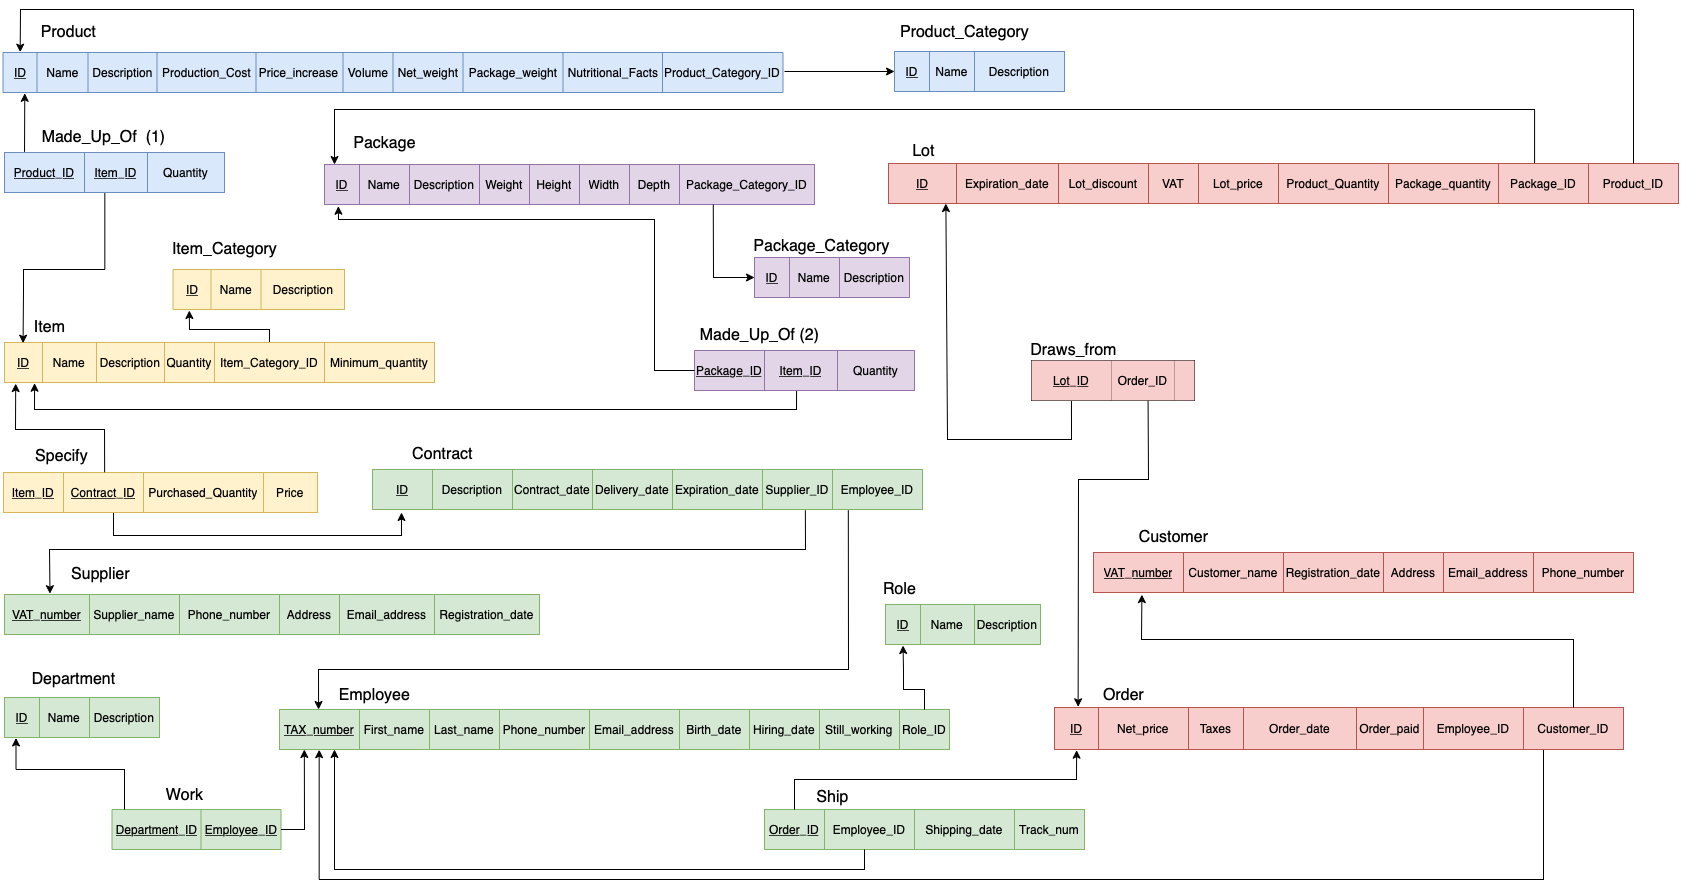
\includegraphics[width=1.3\linewidth,angle=270,origin=c]{Relational.png}
	\caption{Relational schema.}
	\label{fig:relational-schema}
\end{figure}
\newgeometry{margin=25mm}
Ship is a one to many relationship with optional participation either of Order and of Employee, due to the fact that an order can be ready to ship but not been shipped yet and a Worker might not have shipped an order yet. We have created the "Ship" relation, instead of incorporating its attributes into "Order", because if an order is ready but not yet shipped, the "Shipping\_date" and "Track\_num" attributes (as well as the "Employee\_ID" foreing key) would be NULL, and there could be many orders in this situation.
Draws\_from is a one to many relationship with optional participation of Lot, due to the fact that a Lot can be produced in advance (and so it wouldn't be assigned to any order yet). We have created the "Draws\_from" relation, instead of corporating the "Order\_ID" foreing key into Lot because if a Lot is not assigned to any order yet, the "Order\_ID" foreing key would be null, and there could be many lots in this situation.